% ---------------------------------------------------------------------------
% pipelines.tex -- ground-and-solve versus lazy evaluation of the same heuristic.
% Used in the introduction, where the two approaches are first contrasted.
% ---------------------------------------------------------------------------
\documentclass[border=8pt]{standalone}
% ---------------------------------------------------------------------------
% common.tex -- shared preamble for the hand-drawn TikZ diagrams of the thesis.
%
% Every diagram in this folder is a standalone document that inputs this file.
% Change a colour or a style here and it propagates to all figures at the next
% run of ./build.sh.
% ---------------------------------------------------------------------------

\usepackage[T1]{fontenc}
\usepackage{lmodern}
\usepackage{amsmath}
\usepackage{tikz}
\usetikzlibrary{arrows.meta, positioning, fit, backgrounds, calc, shapes.geometric}

% --- palette ---------------------------------------------------------------
\definecolor{diagInk}{RGB}{38,42,50}        % text
\definecolor{diagLine}{RGB}{118,128,142}    % neutral arrows and rules
\definecolor{diagGround}{RGB}{226,233,243}  % ground-and-solve fills
\definecolor{diagGroundEdge}{RGB}{ 96,132,178}
\definecolor{diagLazy}{RGB}{225,240,228}    % lazy fills
\definecolor{diagLazyEdge}{RGB}{ 76,147,100}
\definecolor{diagNeutral}{RGB}{242,242,244} % shared machinery
\definecolor{diagNeutralEdge}{RGB}{150,155,165}
\definecolor{diagAlert}{RGB}{252,232,229}   % the expensive artefact
\definecolor{diagAlertEdge}{RGB}{198, 88, 74}

% --- styles ----------------------------------------------------------------
\tikzset{
  % generic rounded box; the colour is given by one of the *fill styles below
  box/.style={
    draw, rounded corners=2.2pt, line width=0.7pt,
    align=center, inner xsep=7pt, inner ysep=6pt,
    font=\small, text=diagInk, minimum height=9.5mm
  },
  ground/.style={box, fill=diagGround, draw=diagGroundEdge},
  lazy/.style={box, fill=diagLazy,   draw=diagLazyEdge},
  neutral/.style={box, fill=diagNeutral, draw=diagNeutralEdge},
  alert/.style={box, fill=diagAlert,  draw=diagAlertEdge},
  % a box that holds code-like text
  mono/.style={font=\small\ttfamily},
  % arrows
  flow/.style={-{Stealth[length=2.6mm,width=2.0mm]}, draw=diagLine, line width=0.8pt},
  biflow/.style={{Stealth[length=2.6mm,width=2.0mm]}-{Stealth[length=2.6mm,width=2.0mm]},
                 draw=diagLine, line width=0.8pt},
  dashflow/.style={flow, dashed, dash pattern=on 2.6pt off 2.0pt},
  % small caption-like labels
  tag/.style={font=\scriptsize, text=diagInk, inner sep=2pt},
  lane/.style={font=\small\bfseries, text=diagInk},
  % the light band that groups a lane of the diagram
  band/.style={rounded corners=3pt, draw=none, inner sep=9pt},
}


\begin{document}
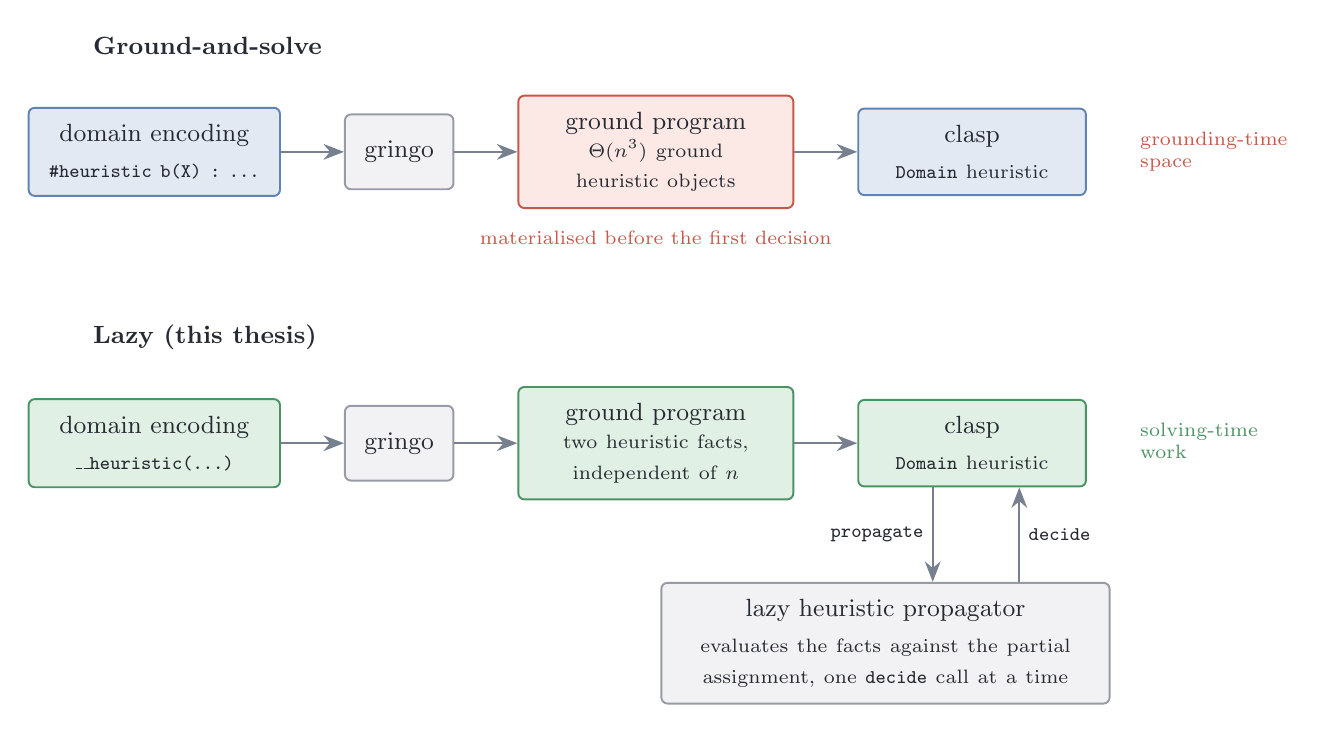
\begin{tikzpicture}

% ======================= ground-and-solve lane =============================
\node[lane, anchor=west] at (0,1.35) {Ground-and-solve};

\node[ground, text width=27mm] (genc) at (0.9,0)
      {domain encoding\\[2pt]{\scriptsize\ttfamily \#heuristic b(X) : \dots}};
\node[neutral, right=8mm of genc]              (ggrin)  {gringo};
\node[alert,   text width=30mm, right=8mm of ggrin] (gprog)
      {ground program\\[2pt]{\scriptsize $\Theta(n^{3})$ ground\\heuristic objects}};
\node[ground,  text width=24mm, right=8mm of gprog] (gclasp)
      {clasp\\[2pt]{\scriptsize \texttt{Domain} heuristic}};

\draw[flow] (genc)  -- (ggrin);
\draw[flow] (ggrin) -- (gprog);
\draw[flow] (gprog) -- (gclasp);

\node[tag, anchor=north, text=diagAlertEdge] at ($(gprog.south)+(0,-2mm)$)
      {materialised before the first decision};

% ============================== lazy lane ==================================
\node[lane, anchor=west] at (0,-2.35) {Lazy (this thesis)};

\node[lazy, text width=27mm] (lenc) at (0.9,-3.7)
      {domain encoding\\[2pt]{\scriptsize\ttfamily \_\_heuristic(\dots)}};
\node[neutral, right=8mm of lenc]              (lgrin)  {gringo};
\node[lazy,   text width=30mm, right=8mm of lgrin] (lprog)
      {ground program\\[2pt]{\scriptsize two heuristic facts,\\independent of $n$}};
\node[lazy,   text width=24mm, right=8mm of lprog] (lclasp)
      {clasp\\[2pt]{\scriptsize \texttt{Domain} heuristic}};

\draw[flow] (lenc)  -- (lgrin);
\draw[flow] (lgrin) -- (lprog);
\draw[flow] (lprog) -- (lclasp);

% the propagator sits underneath the solver and answers its decide calls
\node[neutral, text width=52mm, anchor=north] (prop)
      at ($(lclasp.south)+(-11mm,-12mm)$)
      {lazy heuristic propagator\\[2pt]{\scriptsize evaluates the facts against the
       partial assignment, one \texttt{decide} call at a time}};

\draw[flow] ($(lclasp.south)+(-5mm,0)$) -- ($(lclasp.south)+(-5mm,-12mm)$)
      node[tag, midway, left=1pt] {\texttt{propagate}};
\draw[flow] ($(lclasp.south)+(6mm,-12mm)$) -- ($(lclasp.south)+(6mm,0)$)
      node[tag, midway, right=1pt] {\texttt{decide}};

% =============================== verdict ===================================
\node[tag, anchor=west, text=diagAlertEdge] at ($(gclasp.east)+(6mm,0)$)
      {\begin{tabular}{@{}l@{}}grounding-time\\space\end{tabular}};
\node[tag, anchor=west, text=diagLazyEdge]  at ($(lclasp.east)+(6mm,0)$)
      {\begin{tabular}{@{}l@{}}solving-time\\work\end{tabular}};

\end{tikzpicture}
\end{document}
